\subsection{Mission}
Our mission aside from reaching the marked objective is to attract users.
The user seeks us little we are unique, because we offer something that
Nobody else offers you, because we are different. Sprout among others.
We want the user to trust us, values us, appreciate us, create a link with us. For
We will have to cultivate the relationship and offer a value that provides satisfaction.

To achieve this satisfaction, we have to have a clear mission, which is what we offer, that makes us different.
We can consider what are the characteristics that others do not have, such as more updated and accurate data,
greater coverage of information or a functionality that does not exist up to now, for example, to use the
information that we offer to solve a daily problem.

Once our mission is marked, we face a series of problems, the user may not know that
You need this feature that we provide. We have a double challenge, to offer it to users and
to make him see that it is really necessary, that he helps him in his routine or daily life.

\subsubsection{How to solve it} 
We must study and analyze what gaps the market currently has and what needs the user has.
We will ask ourselves a series of questions, such as how this knowledge can help me.

\subsubsection{How we solve it. Aire Guru} 
The mission of Aire Guru is to increase the awareness of the quality of the air.
There are several problems regarding this issue, the first one is user misinformation, since it is not
aware of the levels of pollution to which it is exposed and on the other hand does not know how it can harm
in the short or long term.

Aire Guru tries to alert the situation, in a way that everyone independent of their cultural level
can understand how air quality influences us. It aims to make available to everyone the knowledge about
This is problematic. How harmful it is to live in a highly polluted area and what are the sources of pollution
more common, so that we can increase awareness and be able to do something about it.


Aire Guru includes in its glossary the most common medical conditions that may be affected by pollution
of the air, the polluting agents and the sources that cause these agents. It is accompanied by an iconography
which reflects each of the symptoms. \\

\begin{figure}[ht]
    \centering
   \subfigure[Glossary detail]
    {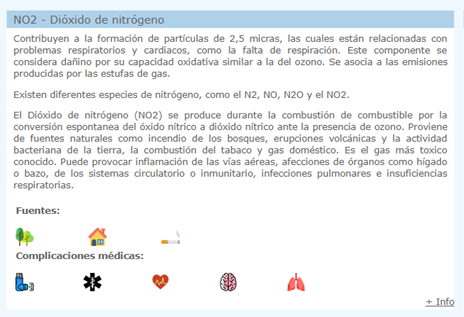
\includegraphics[width=6.2cm  ]{no2_glosary}}
    \hfill
     \subfigure[iconography detail]
     { 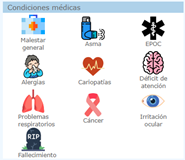
\includegraphics[width=5cm]{iconography}}
  
  \caption{Glossary}
    \end{figure}
\elsparagraph{Evaluation}  
\begin{itemize}
    \done In the survey conducted, users told us that their interest in pollution had grown
         from air. Some of them discovered that they had a medical condition that is affected by the pollution.
    \crossed Air Guru needs more expansion.
    
\end{itemize}
\newpage